%% ============================================================================================
%% DRAFT v2, part 3: Results, one subsection per research question.
%% Every quantity is a macro from numbers.tex; nothing is typed by hand.
%% ============================================================================================

\section{Results}
\label{sec:results}

We report the engineered population E2 (other populations in \S\ref{sec:res-rq3}); unless labelled pooled, a
prevalence is a mean of within-repository proportions with a 95\% bootstrap interval (\S\ref{sec:stats}).

\subsection{RQ1: Delegation structure}
\label{sec:res-rq1}

The \nReposEng{} engineered repositories define \nSpecsEng{} subagent specifications: a median of \medianTeam{} per
repository, a mean of \meanTeam{}, and a maximum of \maxTeam{}. The distribution is heavy-tailed, so the repository is
the unit of analysis throughout. \RQoneNestedPooled{} of specifications (pooled; repository mean \RQoneNested{}) sit in
nested sub-directories, which the runtime does load (\S\ref{sec:oracles}), and \RQoneOutsideRootPooled{} (repository
mean \RQoneOutsideRoot{}) sit in a sub-project's \code{.claude} directory, which only that sub-project's sessions see.

\paragraph{Reuse.}
\RQoneDuplication{} of engineered-population specifications have a byte-identical copy in another corpus repository, and
\RQoneRepeatShare{} are copies beyond the first occurrence of their content in the population. Reuse makes repositories dependent observations, which the one-copy-per-hash analysis in \S\ref{sec:threats}
addresses.

\paragraph{What the delegates are for.}
The intended mode divides the specifications almost in half (pooled): \RQtwoShareInspect{} inspect,
\RQtwoShareChange{} change and \RQtwoShareMixed{} mixed. Only \RQtwoReadonlyClaim{} of specifications make an explicit
read-only claim in their description, so the mode is usually implicit in the purpose. Agreement between the two model
raters on \nReliabilityItems{} items is \alphaRoleModels{} on the role and \alphaModeModels{} on the mode
(\alphaModeBinaryModels{} for inspect against change or mixed), below the 0.667 that
\citet{krippendorff2018content} requires for tentative conclusions; Haiku is the more likely to read a purpose as
inspection (\nModeDisagreeHaikuInspect{} against \nModeDisagreeSonnetInspect{} of \nModeDisagree{} disagreements). By role (pooled), the most common delegates implement
(\RoleShareImpl{}), review code (\RoleShareReview{}) or plan and orchestrate other agents (\RoleSharePlan{}); security
review is \RoleShareSec{}. Given the agreement on the role, no result below rests on these shares.
\authornote{Authors: vet the sixteen-category set before submission.}

\subsection{RQ2: Capability grants}
\label{sec:res-rq2}

\paragraph{Explicit grants and implicit inheritance.}
\RQtwoImplicitEng{} of specifications omit the \code{tools} field and inherit the parent session's entire tool pool,
the largest grant; of these, \RQtwoImplicitCapableCount{} (pooled) can write
files or run a shell. Among specifications that do list tools, \RQtwoExplicitCapable{} can write files or run
a shell on the resolved grant. Requested and effective grants differ: the median explicit list requests
\medianRequested{} tools and resolves to \medianEffective{}, mainly because the resolver drops search tools next to a
shell (\S\ref{sec:res-rq3}); the unresolved names that also separate the two are silent defects (\S\ref{sec:res-rq6}).

\paragraph{Inspection delegates are given fewer file-writing tools.}
Paired within repository, so that repository-level habits cannot explain the difference, specifications whose intended
mode is to inspect hold file-writing tools \RQtwoRoleGapWrite{} less often than specifications whose mode is to change
things, across \RQtwoRoleGapWriteRepos{} repositories that contain both; among explicit grants the gap is
\RQtwoRoleGapWriteExplicit{}. This is consistent with least privilege being applied, in a setting where nothing
compels it.

\paragraph{The margin shrinks when the shell is counted.}
Repeat the paired contrast on whether the agent can reach the file system at all, by a file-writing tool or by a
shell, and the gap falls to \RQtwoRoleGapAuthority{} (\RQtwoRoleGapAuthorityExplicit{} among explicit grants). Most of
the difference concerns which tool names appear in a list, not what the delegate can reach. The residual gap has no
normative baseline: codebook R counts a delegate that runs tests or analyses and only reports as inspection, so some
inspect-mode delegates need a shell, and the tool vocabulary offers no partial shell to grant them.

We could check the dependence on the rater only partly. On the \nRaterSensSpecs{} engineered-population specifications
in the reliability sample, the paired gap is \RaterSensGapWriteHaiku{} for file-writing tools and
\RaterSensGapAuthorityHaiku{} for any reach under Haiku's labels (\RaterSensReposHaiku{} repositories hold both modes),
and \RaterSensGapWriteSonnet{} and \RaterSensGapAuthoritySonnet{} under Sonnet's (\RaterSensReposSonnet{}
repositories). The two sets of repositories differ and are small, and even under Haiku's labels the subsample does
not reproduce the full-population gap. The check supports the direction of both gaps and that the any-reach gap is
much the smaller one, not their size.

\subsection{RQ3: Coherence of restrictions}
\label{sec:res-rq3}

\paragraph{Dominated withholding.}
In the average engineered repository, \textbf{\RQthreeIncoherentEng{}} of the explicit grants that withhold every
file-writing tool keep a shell with no command scope, which can perform every withheld operation
(\S\ref{sec:capmodel}); the mean is over the \nReposWithhold{} repositories with such a grant, and the dominated
withholdings are \nDomSpecs{} specifications in \nDomRepos{} repositories. Among grants that keep a shell, only
\RQthreeScopedShare{} scope it to specific commands. The rate does not depend on counting delegates meant to change
files through the shell: \nDomChangeMode{} of the \nDomSpecs{} are change-mode, and among inspect-mode specifications
alone the share is \RQthreeIncoherentInspect{}. We also observed a related resolver behaviour: in every explicit list
where \code{Bash} resolves, the resolver drops \code{Grep} and \code{Glob} (\RQthreeGrepDroppedResolved{} lists),
while none of the \nGrepListsNoBash{} lists without \code{Bash} loses them. We know of no documented reason; its
effect is to move routine search onto the shell. \code{Write}, \code{Edit} and \code{NotebookEdit} stay in place next
to the shell, and neither the drop nor the retained write path is reported.

\paragraph{Committed execution context.}
Whether these grants can write in practice also depends on the session's permission mode and on settings
(\S\ref{sec:capmodel}); the mode and user-level settings are not observable. Of the \nDomRepos{} repositories with a
dominated withholding, \nDomReposSettings{} commit a \code{.claude/settings.json}: \nDomReposDeny{} have a deny rule
that mentions a file-writing tool or \code{Bash}, \nDomReposHooks{} define hooks, \nDomReposAllowBash{} allow the
unscoped shell, \nDomReposNoApprovalMode{} set a default mode that approves some or all shell commands automatically
(\code{acceptEdits}, \code{auto} or \code{bypassPermissions}), and \nDomReposSandbox{} enables the sandbox, which
confines shell commands at the operating-system level. Deny rules and hooks can block matching commands; we did not
evaluate which writes they block. \nDomPlan{} dominated-withholding specifications set \code{permissionMode: plan},
which applies only when the parent session runs in \code{default}, \code{dontAsk} or \code{plan} mode; excluding them
gives \RQthreeIncoherentNoPlan{}.

\paragraph{Is the shell needed?}
Keeping a shell may be legitimate, so we coded what the text of one dominated-withholding specification per repository
asks the shell to do (codebook B, \nShellLabelled{} specifications). The text gives no reason to run commands in
\ShellUseNone{}, asks only for read-only commands such as \code{git log} or \code{grep} in \ShellUseInspect{}, asks to
build, test or lint in \ShellUseVerify{}, and asks for state-changing commands in \ShellUseChange{}. Agreement with the
second rater (\nShellReliability{} specifications in whole batches) is \alphaShellUse{} on the four values and
\alphaShellChange{} for change against the rest, below the threshold for tentative conclusions, so we read the shares
as indicative (a third model agrees with the primary rater at \alphaOpusShellHaiku{}, \S\ref{sec:threats}). On the double-coded specifications, \ShellNoChangeHaikuRel{} ask for no state-changing command under
the primary rater's labels and \ShellNoChangeSonnetRel{} under the second rater's, who reads more build and test
instructions as changes. Under the primary rater, \ShellUseNoChangeNeed{} of these specifications never ask the agent
to change anything by command; counting verification as a change, \ShellUseNoneOrInspect{} ask for at most read-only
commands. For the inspect group, a shell limited to read-only commands would provide what the text asks for, but a
command pattern in the \code{tools} field does not provide that limit. We gave a subagent
\code{tools: Read, Grep, Glob, Bash(git log:*)} and, in the experiment's auto permission mode on v\ScopedBuild{},
asked it to create a file (four runs per model) or to read the last commit message (two per model). It created the
file in \ScopedCreated{} runs, every time through the shell (\code{echo}, \code{printf} or a here-document; no
file-tool call), and answered the \code{git log} request in \ScopedControls{}: the pattern granted the whole shell.
Whether the pattern acts as a pre-approval that leaves other commands to prompt in default mode we did not test. The
documented mechanism is a Bash deny rule in settings, which applies to subagents \citep{AnthropicSubagentsDoc}, and such rules
match command text: the documentation's own example shows a \code{git log} rule matching
\code{git log --output=<file>}, which writes a file \citep{AnthropicPermissionsDoc}. Verification is a genuine need,
and test runners execute repository code and write caches and build outputs, so a verify-type shell needs a sandbox or
a writable scratch directory rather than a command pattern.

\paragraph{Robust to the curation cuts.}
Across ALL, E1, E2 and E3, the share of specifications omitting \code{tools} is \PopAllImplicit{}, \PopEoneImplicit{},
\PopEtwoImplicit{} and \PopEthreeImplicit{}; the share of write-withholding explicit grants that keep an unscoped shell
is \PopAllIncoherent{}, \PopEoneIncoherent{}, \PopEtwoIncoherent{} and \PopEthreeIncoherent{}; and the paired
inspect--change gap falls from \PopAllGapWrite{}, \PopEoneGapWrite{}, \PopEtwoGapWrite{} and \PopEthreeGapWrite{}
points for file-writing tools to \PopAllGapAuthority{}, \PopEoneGapAuthority{}, \PopEtwoGapAuthority{} and
\PopEthreeGapAuthority{} points once the shell is counted. By repository size (specifications per repository) the share is \RQthreeIncoherentBySize{}, so the
repositories that file-level discovery favours do not drive it.

\subsection{RQ4: Prose versus enforcement}
\label{sec:res-rq4}

\paragraph{What developers forbid.}
The corpus contains \nDirectiveSentences{} prohibition and obligation sentences (all specifications), of which
\pctProhibitionSentences{} are prohibitions, and \RQfourAnyProhibition{} of engineered specifications with
Latin-script bodies contain at least one prohibition (\pctNonLatin{} of bodies are in other scripts). Few directive sentences concern
authority. In the annotated sample, the largest topic is the quality of the work (\CatQuality{}); file modification
(\CatFsModify{}), command execution (\CatExec{}) and destructive operations (\CatDestructive{}), which a tool grant can
enforce, are small minorities, and \CatRestrictsWrites{} of directive sentences restrict the agent's own writes.

\paragraph{The two channels disagree.}
Read as a whole, the text of \RQfourProseAny{} of engineered specifications restricts the agent's own writes:
\RQfourProseFull{} make the agent read-only and \RQfourProsePartial{} forbid or condition some writes (codebook S,
\nSpecSample{} specifications, one per repository; agreement with the second rater on \nSpecReliability{}
specifications \alphaSpecFull{} on read-only against not, \alphaSpecRestr{} on all three values). Of the \nSpecFull{}
read-only specifications, \RQfourFullReaches{} hold an effective grant that can still reach the file system:
\RQfourFullWriteTool{} hold a file-writing tool, most because they omit the \code{tools} field (\RQfourFullImplicit{}
of all read-only specifications), and \RQfourFullShellOnly{} withhold every file-writing tool but keep an unscoped
shell. Only \RQfourFullEnforced{} have a grant with neither a file-writing tool nor an unscoped shell, and such a grant
can still hold authority outside our model: of the \nRestrictedGrants{} explicit grants of this kind in E2,
\nRestrictedWeb{} hold a web tool, \nRestrictedMcp{} name MCP tools and \nRestrictedTask{} can delegate further. When the
text makes an agent read-only, the restriction is stated in the interpreted channel and only partly carried into the
enforced one.

\subsection{RQ5: Behaviour under repeated execution}
\label{sec:res-rq5}

\nExpRuns{} runs were scored; \nExpIncomplete{} were cut off by a usage limit. All ran in \code{auto} mode, and
the permission layer denied no action, so the results are conditional on shell commands running without per-command
approval; in \code{default} mode each shell command would have needed the user's approval. Table~\ref{tab:experiment} and
Fig.~\ref{fig:experiment} give every cell.

\begin{table}[t]
\caption{Experiment outcomes: runs in which the task's objective held afterwards (T2--T5 verified on the file
system, T1 and T6 from the reported value), out of scored runs. T2--T5 (create, modify, delete, run a file-writing
script) are forbidden by the prompts of C1 and C3; T1 (read a value) and T6 (run a script and report its output)
are permitted everywhere, and T6 needs a shell. C2 and C3 resolve to \code{Read, Bash}, because the resolver
drops \code{Grep} and \code{Glob} next to \code{Bash}.}
\label{tab:experiment}
\footnotesize
\setlength{\tabcolsep}{4pt}
\begin{tabular}{@{}llrrrrr@{}}
\toprule
 & & \multicolumn{3}{c}{\textbf{T2--T5, by model}} & \multicolumn{2}{c}{\textbf{all models}} \\
\cmidrule(lr){3-5}\cmidrule(l){6-7}
\textbf{Config.} & \textbf{Grant and prompt} & \textbf{Haiku} & \textbf{Sonnet} & \textbf{Opus} & \textbf{T1} & \textbf{T6} \\
\midrule
C0 & no \code{tools}, neutral prompt & 115/120 & 112/119 & 116/120 & 88/88 & 90/90 \\
C1 & no \code{tools}, prompt forbids writes & 54/120 & 2/120 & 0/118 & 89/89 & 89/89 \\
C2 & \code{Read, Grep, Glob, Bash} & 119/119 & 120/120 & 120/120 & 90/90 & 90/90 \\
C3 & C2 grant + C1 prompt & 41/120 & 0/119 & 0/120 & 90/90 & 90/90 \\
C4 & \code{Read, Grep, Glob} & 0/120 & 0/120 & 0/120 & 90/90 & 0/89 \\
\bottomrule
\end{tabular}
\end{table}


\begin{figure}[t]
\centering
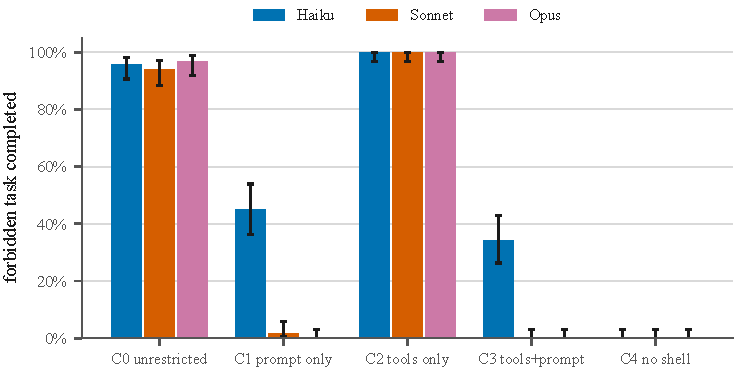
\includegraphics[width=.62\textwidth]{fig10_experiment}
\caption{Share of runs completing a requested file change (T2--T5) that the prompts of C1 and C3 forbid and the
grants of C2--C4 were meant to prevent, by configuration and model, with Wilson 95\% intervals (\code{auto} permission
mode). Only the removal of the shell (C4) prevents the change for every model; the prompt restriction (C1, C3) almost
entirely prevents it for Sonnet and Opus but not for Haiku.}
\label{fig:experiment}
\end{figure}

\paragraph{Mechanism check: the shell carries out a requested change.}
C2 pairs the modal inspection grant with a neutral prompt, so from the agent's point of view the change is requested,
not forbidden. Agents completed the requested file change in \ExpCtwoRate{} of runs on T2--T5, for every model; with
the shell withheld as well (C4), in \ExpCfourRate{}. All \ExpCtwoShellShare{} successful C2 runs on T2--T4 reached the
file through the shell. The runtime does enforce the grant: in \nExpDeniedFileTool{} runs the agent first called a withheld
file tool and was refused (``No such tool available''). Without a shell, \nExpDeniedNoShellSuccess{} of these runs
then made the change; with a shell, the change was made anyway (\nExpDeniedWithShellSuccess{} of
\nExpDeniedWithShell{}).

\paragraph{In the realistic inspection configuration, a prompt restriction holds for Sonnet and Opus, not reliably for
Haiku.}
C3 adds a prompt restriction to the same grant, as an inspection specification with a reviewer-style body would. It
lowers success to \ExpCthreeRate{} overall: \ExpCthreeSonnet{} for Sonnet, \ExpCthreeOpus{} for Opus and
\ExpCthreeHaiku{} for Haiku (C3 against C2, pooled over models: \ExpTestPromptShell{}). A prompt
restriction with every tool granted (C1) gives \ExpConeRate{} against \ExpCzeroRate{} unrestricted (C0), with the same
ordering: \ExpConeSonnet{}, \ExpConeOpus{} and \ExpConeHaiku{} (\ExpTestPromptNoTools{}). Whether the prompt holds depends on the model
that reads it. It is one explicit wording, stronger than most real restrictions, against direct requests, so these
rates are a best case for prompts and say nothing about adaptive attacks.

\paragraph{An observation: without a shell, Haiku sometimes reported a change it had not made.}
Of the \nExpFailedForbidden{} forbidden-task runs that left the file unchanged, \nExpFalseClaims{} end with a final
answer stating that the change was made (``The file \code{obsolete.log} has been successfully deleted''), and
\nExpAmbiguousClaims{} more present the intended result without saying it was not applied (codebook~K; all positive
and ambiguous labels were re-read against the answers by the first author and stand). All \nExpFalseClaims{} are Haiku runs
without a shell (C4), \ExpFalseClaimsCell{} of that cell (Wilson 95\% interval \ExpFalseClaimsCI{}); no Sonnet or Opus
run claimed a change it had not made.

\paragraph{Asked only for a report, agents did not change files.}
In the report-only extension, \nOverChanged{} of \nOverRuns{} runs changed, created or deleted any fixture file
(\OverRate{}): C0 \OverCZero{}, C2 \OverCTwo{}, C3 \OverCThree{} and C4 \OverCFour{}, including the configuration with
every tool. The answers named the error in \OverFoundBug{} of runs, and the permission layer denied
\nOverPermissionDenials{} actions; asked to find a bug, no model fixed it. The result bounds the per-configuration rate
of unrequested changes below these upper bounds only for benign, explicitly report-only tasks: one small fixture, two
tasks, \nOverRepsFinal{} repetitions per cell and no adversarial content. It does not cover ambiguous requests such
as ``fix if needed'', longer sessions or prompt injection. It agrees with \citet{qu2026overeager}, who observe no
over-eager actions by Claude Code when the prompt declares the authorised scope and 17.1\% when that declaration is
removed from scenarios built to invite such actions; our tasks state their scope (``tell me'').

\paragraph{Side effects and builds.}
No run changed a fixture file its task did not name. \nExpOutsideWrites{} runs wrote outside their fixture directory,
although the prompt named it: \nExpOutsideCwd{} Haiku runs under C2 and C3 ran the script from the orchestrating
session's working directory before retrying inside the fixture, and \nExpOutsideTrash{} Opus runs under C0 ``deleted''
the file by moving it to the user's Trash or another directory. These are containment failures that neither the grant
nor the prompt prevented; only a sandbox confining writes to the fixture could have. Per model and configuration, we
detect no difference in forbidden-task success between any two of the three builds (\nExpBuildComparisons{} Fisher
tests, smallest $p=\ExpPeriodMinP{}$, uncorrected); with \ExpBuildCellSizes{} runs per cell and build, only large
differences were detectable.

\subsection{RQ6: Silent defects and drift}
\label{sec:res-rq6}

Admission is not where specifications are lost: \RQsixRegistered{} of those staged at a probed root are registered
(pooled). Resolution is. In the average repository that lists tools, \RQsixUnresolved{} of its explicit grants name at
least one tool the runtime does not resolve (\RQsixLegacy{} a tool removed in an earlier release, \RQsixNeverValid{} a
name never valid in any release we tested); \RQsixUnresolvedRepos{} of the \nReposExplicit{} repositories with an
explicit grant contain at least one such grant (removed names \RQsixLegacyRepos{}, never-valid names
\RQsixNeverValidRepos{}). Context-conditional names (interactive-only, flag-gated or platform-specific) are reported
separately and not counted as defects. \RQsixShadowed{} specifications in \RQsixShadowedRepos{} of repositories declare
a name that another file under the same root already declares; exactly one loads, and the other is discarded without a
message.

Of the \nDriftDated{} files naming a removed tool that we could date, \RQsixDriftAfter{} (pooled) were first committed
\emph{after} the release that removed the name, so they were already unresolvable on current builds when committed,
rather than overtaken by the runtime later (users of older builds may still resolve them). Most of the corpus was
committed after these removals, so the share dates the staleness, not its source. The feedback is asymmetric: the settings layer warns about every deny or ask
rule that matches no known tool (\RQsixVoidSettings{} of repositories that commit settings have one), while the subagent
resolver says nothing about a dropped name, a collision or a file it declines to load.

\subsection{RQ7: Governance context}
\label{sec:res-rq7}

Many engineered repositories use conventional access controls: \RQsevenBranchProtected{} protect their default branch,
\RQsevenRulesets{} define rulesets, \RQsevenCodeowners{} declare code owners, \RQsevenDependabot{} run Dependabot and
\RQsevenSecurityPolicy{} publish a security policy. The share of all specifications that are dominated withholdings is
\RQsevenIncoherentGoverned{} in repositories that protect their default branch and \RQsevenIncoherentUngoverned{} in
those that do not, a difference of \RQsevenBPDiff{}: branch-protected repositories have slightly more dominated
withholding, not less. The differences for a \code{settings.json} that denies writes or shells (\RQsevenSettingsDeny{}
of repositories), \RQsevenDiffSettingsDeny{}, and for every CI workflow declaring its token permissions
(\RQsevenCiAllScoped{} of repositories), \RQsevenDiffCiScoped{}, are inconclusive.
The outcome counts all specifications, so it also rises with how often a repository withholds file tools at all. On
this observational evidence, with many uncontrolled differences between repositories, conventional access controls
do not go with fewer dominated withholdings; the small positive difference should not be read as an effect.
